\index{keywords}{Installation}RGG installers can be obtained at \url{http://www.computationalmodelbuilder.org/download/} for all three major operating systems: Windows, Mac OS X, and Linux.  Detailed installation guides are detailed below by platform.

\section{Windows}
\index{keywords}{Windows Installation}
A security warning may come up and ask for permission to allow the installer to make changes to your computer.  Be sure to click \ui{Yes}[Windows Installer] to allow the installation process to continue.  This may require authentication by your computer's administrator.

A window like Figure \ref{fig:WindowsInstall1} should come up.

\begin{figure}
\centering
\begin{minipage}{.40\textwidth}
  \centering
	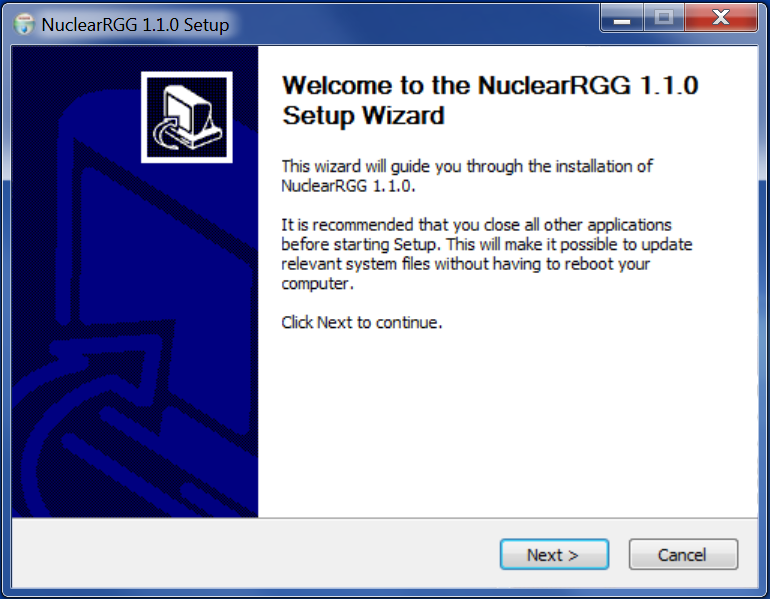
\includegraphics[width=0.90\linewidth]{Images/windows-install-1.png}
	\caption{Beginning the installation process.}
	\label{fig:WindowsInstall1}
\end{minipage}%
\begin{minipage}{.40\textwidth}
  \centering
	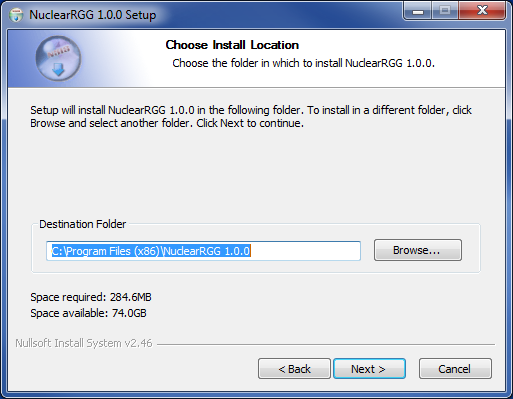
\includegraphics[width=0.90\linewidth]{Images/windows-install-2.png}
	\caption{Selecting the install location.}
	\label{fig:WindowsInstall2}
\end{minipage}
\end{figure}

Click \ui{Next}[Windows Installer] to continue and agree to the license displayed.  On the next screen (shown below), either use the default install location or select one of your own (Figure \ref{fig:WindowsInstall2}.  Click \ui{Next}[Windows Installer].

On the next window (shown below), select whether or not you'd like a Start Menu Folder to be created for RGG.  If you would not link a Start Menu Folder to be created, select the \ui{Do not create shortcuts box}[Windows Installer].  Otherwise, confirm the Start Menu Folder name you'd like to use (Figure \ref{fig:WindowsInstall3}.  Click install to have the installer extract the binaries.

\begin{wrapfigure}{r}{0.40\textwidth}
	\begin{center}
		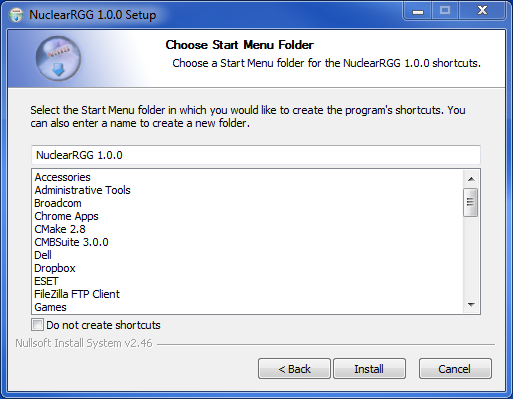
\includegraphics[width=0.9\linewidth]{Images/windows-install-3.png}
		\caption{Configuring Start Menu Folders.}
		\label{fig:WindowsInstall3}
	\end{center}
\end{wrapfigure}

A window should come up to confirm that RGG has been successfully installed on your computer.  At this point, you can click \ui{Finish}[Windows Installer] to close this wizard.

\section{Mac}
\toIndex{Mac Installation}
We use a standard drag and drop installer on Mac.  Simply mount the .dmg file and drag the RGG app into the Applications folder alias.

\section{Linux}
\toIndex{Linux Installation}
We provided a self-contained tar.gz file.  To install, one extracts the folder and places it contents.  In order for the executable to run, the bin and lib file must be at the same directory level.
